\documentclass[10pt]{beamer}

\usetheme[progressbar=frametitle]{metropolis}
\usepackage{appendixnumberbeamer}

\usepackage{booktabs}
\usepackage[scale=2]{ccicons}

\usepackage{pgfplots}
\usepgfplotslibrary{dateplot}

\usepackage{xspace}
\newcommand{\themename}{\textbf{\textsc{metropolis}}\xspace}
\newcommand{\bol}[1]{\textbf{#1}}

\title{Non-linear Dimensionality Reduction}
\subtitle{t-Distributed Stochastic Neighbor Embedding}
% \date{\today}
\date{}
\author{Xiaoyu Xue}
\institute{Microsoft BingAds UCM}
% \titlegraphic{\hfill\includegraphics[height=1.5cm]{logo.pdf}}
 \metroset{block=fill}
\begin{document}

\maketitle

\begin{frame}{Table of contents}
  \setbeamertemplate{section in toc}[sections numbered]
  \tableofcontents[hideallsubsections]
\end{frame}

\section{Dimensionality Reduction}
\begin{frame}{Dimensionality Reduction}
\begin{block}{Definition of dimensionality reduction:}
Given a set of data $X = [\bold{x}_1,\ldots,\bold{x}_m]$, $\bold{x}_i \in \mathbb{R}^n$, find a map $f: \mathbb{R}^n \to \mathbb{R}^d$, make $\bold{y}_i = f(\bold{x}_i) \textrm{ and } d\ll n$. Where $f = (f_1, \ldots, f_n)$, $f_i: \mathbb{R}^n \to \mathbb{R}$
\end{block}
\bigskip
\begin{block}{Linear Dimensionality Reduction}
If $f_i$ is a linear map, $f = P = [\bold{p}_1, \ldots, \bold{p}_n], \bold{y}_i = P^T\bold{x}_i$
\end{block}
\end{frame}

\begin{frame}{Dimensionality reduction: Some Assumptions }
\begin{enumerate}
\setlength{\itemsep}{5pt}
\setlength{\parsep}{5pt}
\setlength{\parskip}{5pt}
	\item High-dimensional data often lies on or near a much lower dimensional, curved manifold 
	\item A good way to represent data points is by their low-dimensional coordinates.
	\item The low-dimensional representation of the data should capture information about high-dimensional pairwise distances. 
\end{enumerate}
\end{frame}

\begin{frame}{Dimensionality Reduction}
\begin{itemize}
\setlength{\itemsep}{12pt}
\setlength{\parsep}{12pt}
\setlength{\parskip}{12pt}
	\item \textbf{Linear Dimensionality Reduction}: PCA(Principal Components Analysis), LDA(Linear Discriminant Analysis), MDS(Classical Multidimensional Scaling) 
	\item \textbf{None-Linear Dimensionality Reduction}: Isomap(Isometric Mapping), LLE(Locally Linear Embedding), LE(Laplacian Eigenmaps), \textbf{tSNE}(t-Distributed Stochastic Neighbor Embedding)
\end{itemize}
\end{frame}

\section{Stochastic Neighbor Embedding}
\begin{frame}{Stochastic Neighbor Embedding}
Define the similarity of data point $\bold{x}_i$ in original space as conditional probability $p_{j|i}$. It is the probability that $\bold{x}_i$ would pick $\bol{x}_j$ as its neighbor under a Gaussian centered at $\bol{x}_i$
\begin{displaymath}
	p_{j|i} = \frac{\exp{(-\Vert\bol{x}_i - \bol{x}_j\Vert^2 / 2\sigma_i^2)}}{\sum_{k \neq i}\exp(-\Vert\bol{x}_i - \bol{x}_k\Vert^2 / 2\sigma_i^2)}
\end{displaymath}
\begin{figure}
\centering
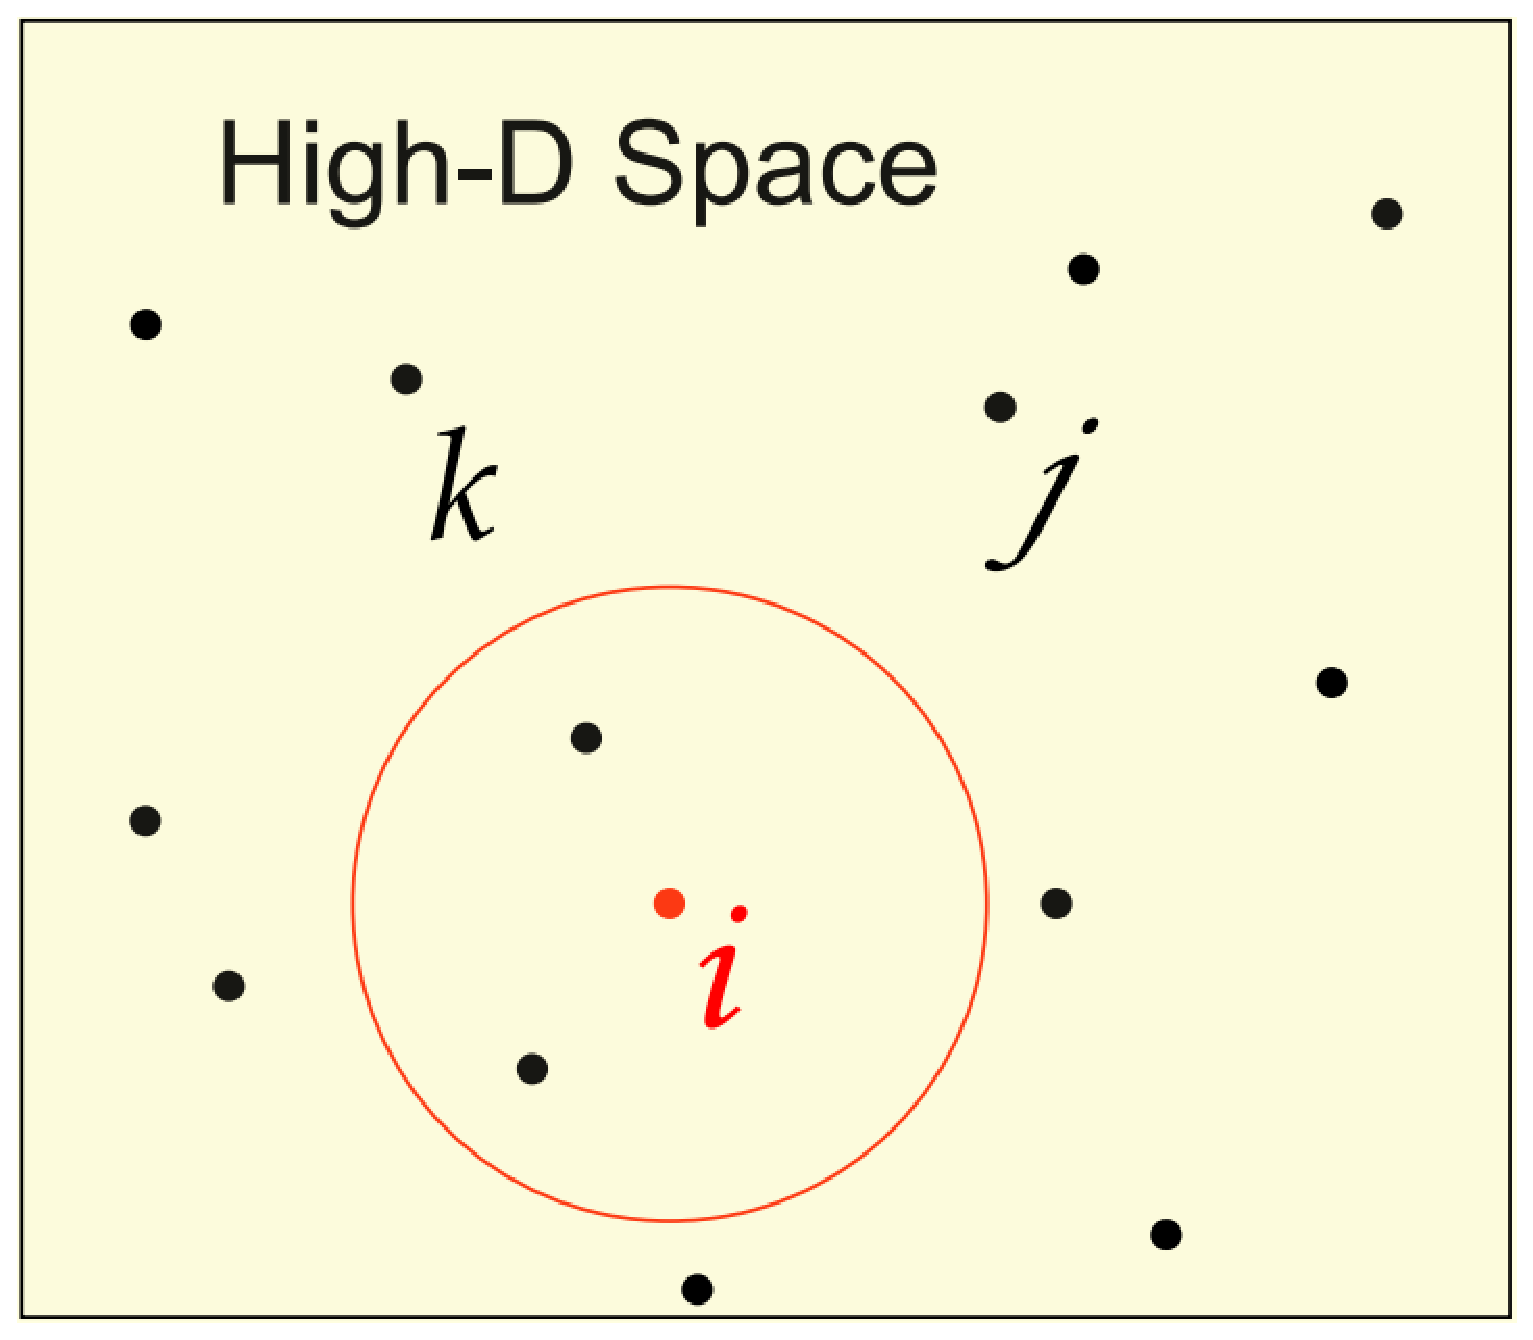
\includegraphics[scale=0.2]{./image/hd.eps}
\end{figure}
\end{frame}


\begin{frame}{Stochastic Neighbor Embedding}
In low-dimensional space, define the similarity $q_{j|i}$
\begin{displaymath}
	q_{j|i} = \frac{\exp{(-\Vert\bol{y}_i - \bol{y}_j\Vert^2)}}{\sum_{k \neq i}\exp(-\Vert\bol{y}_i - \bol{y}_k\Vert^2)}
\end{displaymath}
\begin{figure}
\centering
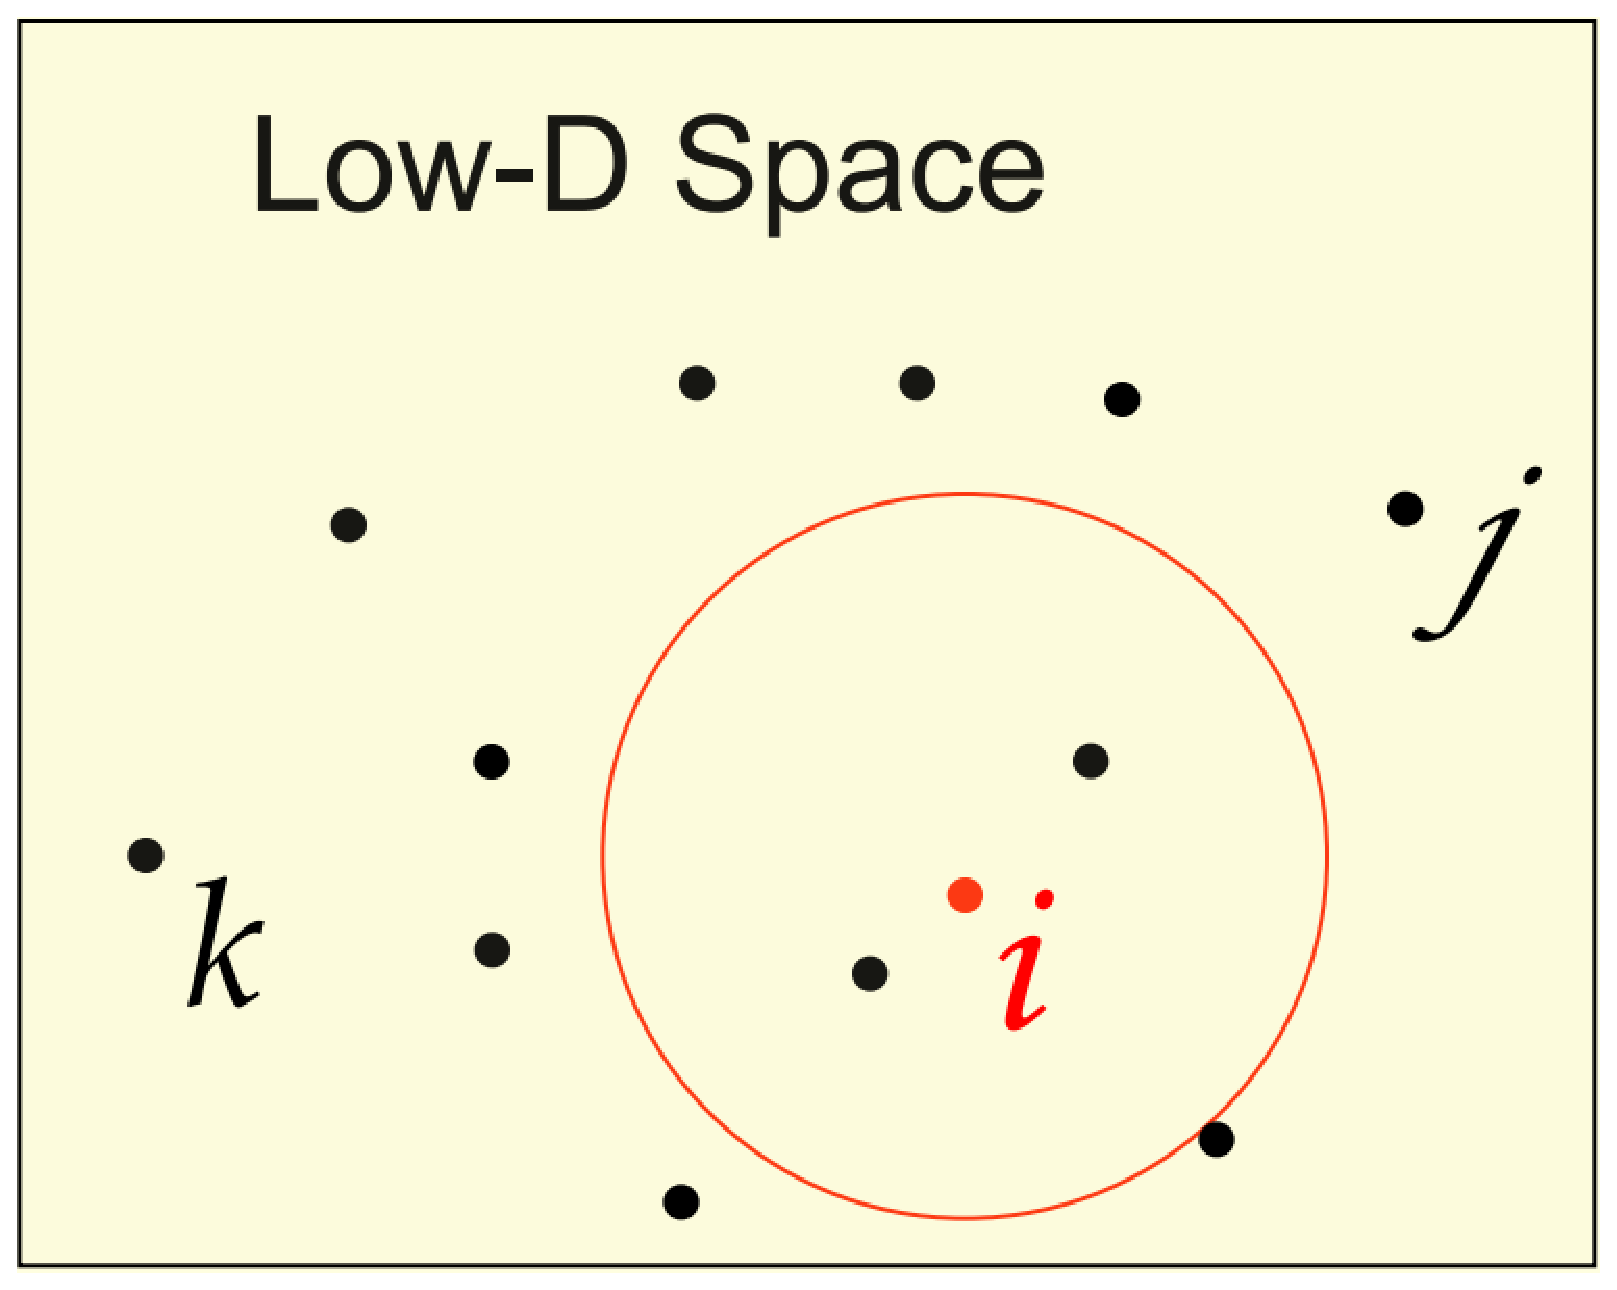
\includegraphics[scale=0.2]{./image/ld.eps}
\end{figure}
\end{frame}


\begin{frame}{Cost function of SNE}
If the map points $\bol{y}_i$ and $\bol{y}_j$ correctly model the similarity between the high-diminsional datapoints $\bol{x}_i$ and $\bol{x}_j$, the conditional probability $p_{j|i}$ and $q_{j|i}$ will be equal. Use the Kullback-Leibler divergences to minimize the mismatch:
\begin{displaymath}
	Cost = \sum_i KL(P_i||Q_i) = \sum_i\sum_j p_{j|i} \log\frac{p_{j|i}}{q_{j|i}}
\end{displaymath}
To minimize the cost function using gradient descent:
\begin{displaymath}
	\frac{\partial Cost}{\partial \bol{y}_i} = 2\sum_j (p_{j|i} - q_{j|i} + p_{i|j} - q_{i|j})(\bol{y}_i - \bol{y}_j)
\end{displaymath}
\end{frame}


\begin{frame}{Stochastic Neighbor Embedding}
About the cost function:
\begin{displaymath}
	Cost = \sum_i KL(P_i||Q_i) = \sum_i\sum_j p_{j|i} \log\frac{p_{j|i}}{q_{j|i}}
\end{displaymath}
\begin{itemize}
	\item Large $p_{j|i}$ modeled by small $q_{j|i}$, Big penalty !
	\item Small $p_{j|i}$ modeled by large $q_{j|i}$, Small penalty ! 
	\item It is asymmetric and mainly preserves local similarity structure of data !
\end{itemize}
\end{frame}

\begin{frame}{Stochastic Neighbor Embedding}
The ``Crowding'' problem
\begin{itemize}
	\item Try to model the local structure of data in the map !
	\item Dissimilar points have to be modeled  as too far apart in the map !
	\item SNE does not have gaps between classes !
\end{itemize}
\begin{figure}
\centering
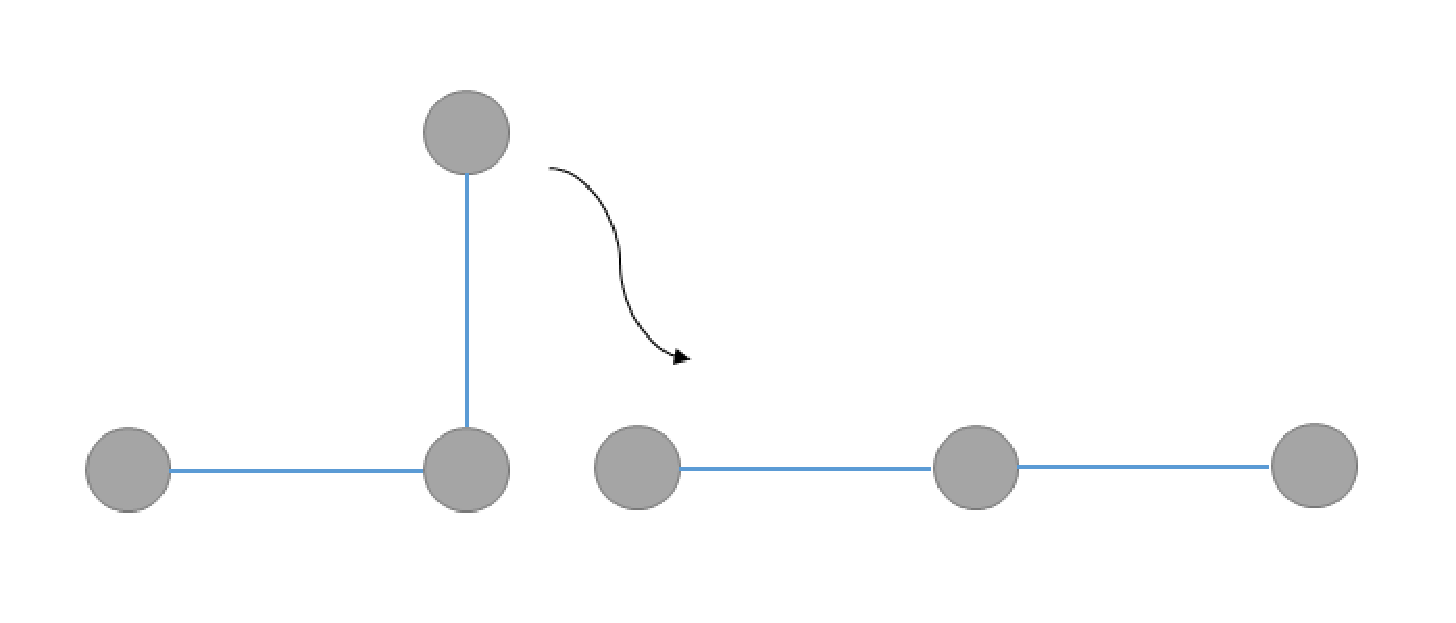
\includegraphics[scale=0.35]{./image/tsne1.eps}
\end{figure}
\end{frame}

\begin{frame}{Stochastic Neighbor Embedding}
\begin{figure}
\centering
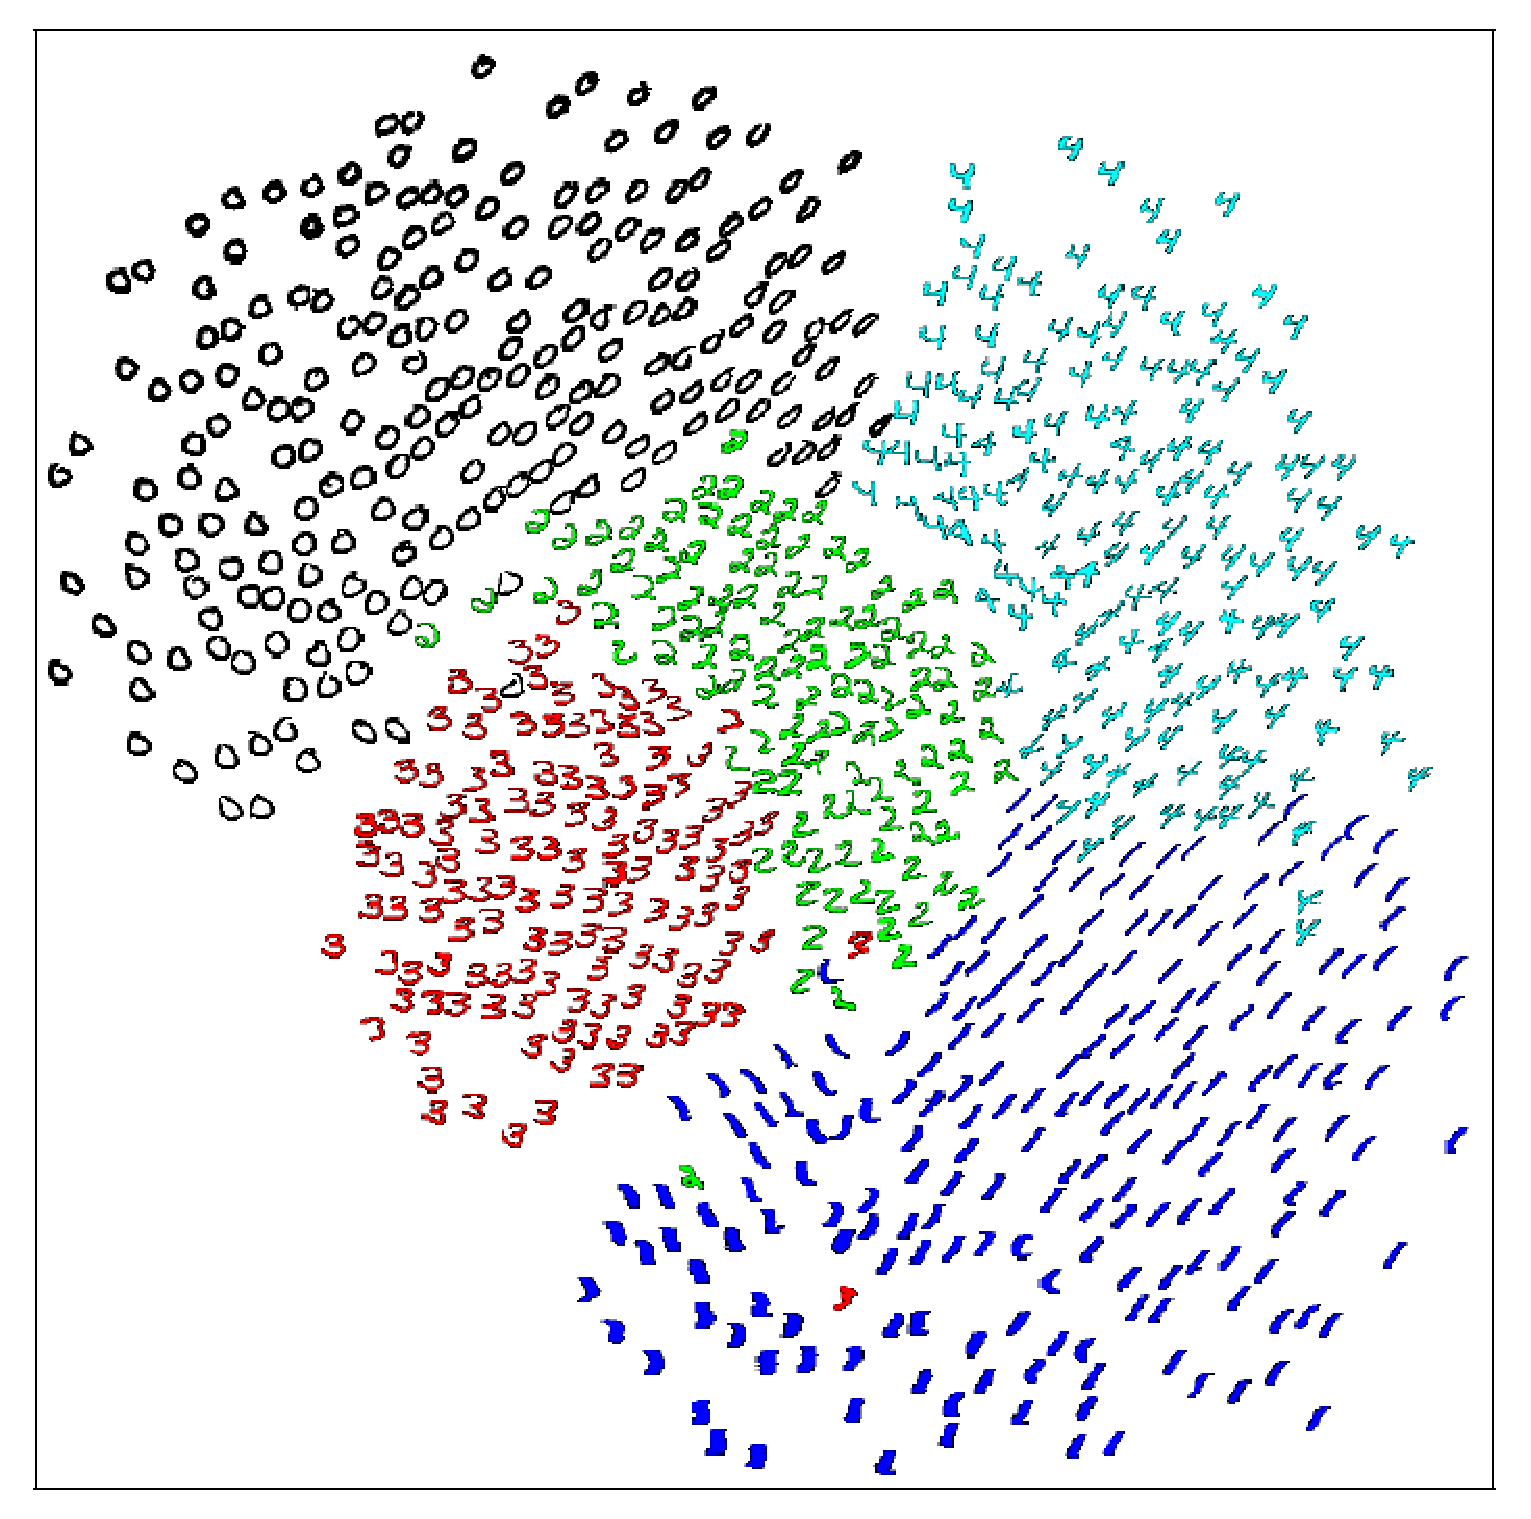
\includegraphics[scale=0.3]{./image/sne.eps}
\end{figure}
\end{frame}
\section{t-Distributed Stochastic Neighbor Embedding}
\begin{frame}{t-Distributed Stochastic Neighbor Embedding}
Symmetric SNE by using joint probability distribution instead of conditional probability distribution.
\begin{displaymath}
	p_{ij} = \frac{p_{i|j} + p_{j|i}}{2m}
\end{displaymath}
Cost function becomes:
\begin{displaymath}
	Cost =  KL(P||Q) = \sum_i\sum_j p_{ji} \log\frac{p_{ji}}{q_{ji}}
\end{displaymath}
\end{frame}


\begin{frame}{t-Distributed Stochastic Neighbor Embedding}
Use t distribution (Heavy-tailed distribution) to model similarity in low-dimensional space to release the ``Crowding'' problem
\begin{figure}
\centering
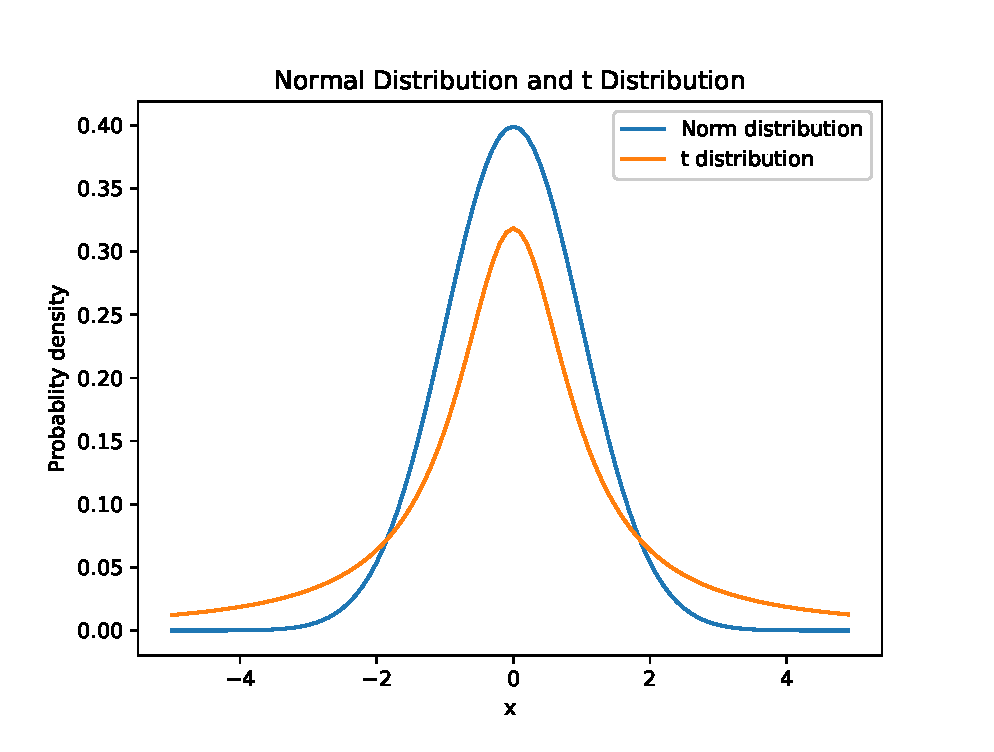
\includegraphics[scale=0.5]{./image/tsne2.eps}
\end{figure}
\end{frame}


\begin{frame}{t-Distributed Stochastic Neighbor Embedding}
The joint probabilities $q_{ij}$ are defined as
\begin{displaymath}
	q_{ij} = \frac{(1 + \Vert \bol{y}_i - \bol{y}_j \Vert^2)^{-1}}{\sum_{k !=l}(1 + \Vert \bol{y}_k - \bol{y}_l \Vert^2)^{-1}}
\end{displaymath}
\begin{figure}
\centering
\includegraphics[scale=0.45]{./image/tsne5.eps}
\end{figure}
\end{frame}


\section{Hardwriting digit visualization}
\begin{frame}{Hardwriting digit visualization}
\begin{figure}
\centering
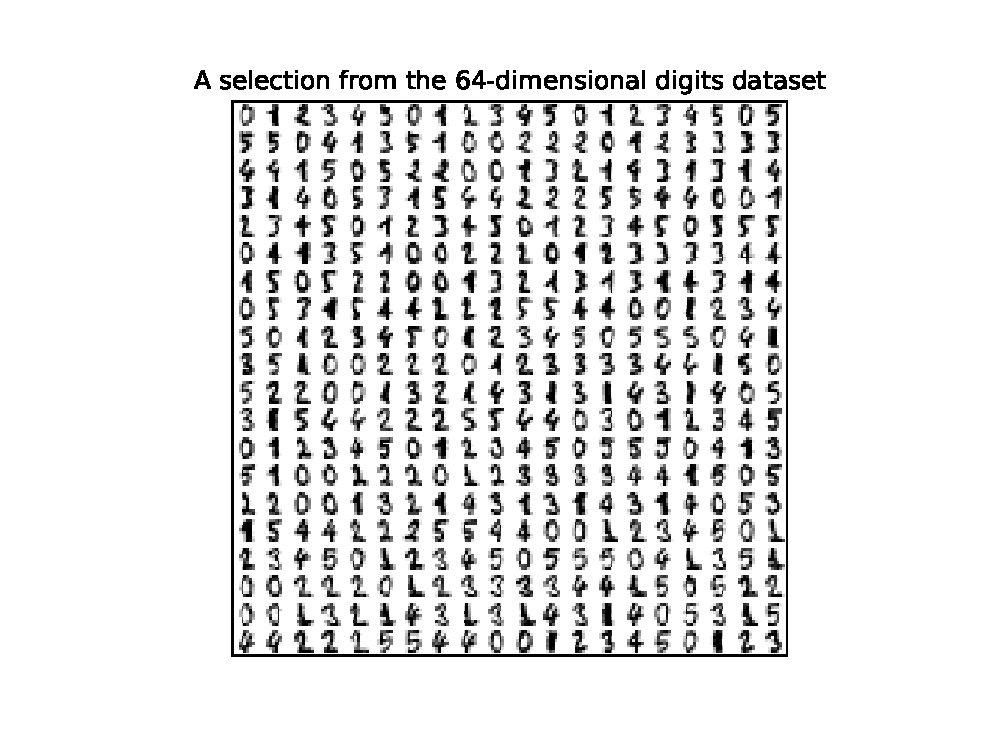
\includegraphics[scale=0.65]{./image/experiment/example.eps}
\end{figure}
\end{frame}


\begin{frame}{Hardwriting digit visualization}
\begin{figure}
\centering
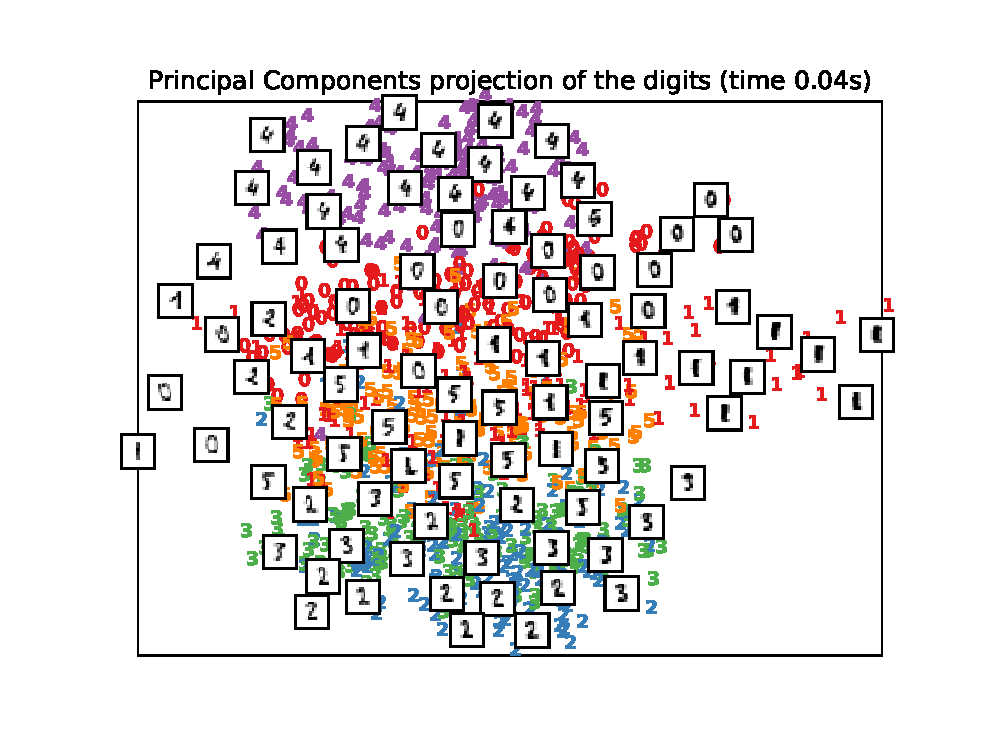
\includegraphics[scale=0.65]{./image/experiment/pca.eps}
\end{figure}
\end{frame}


\begin{frame}{Hardwriting digit visualization}
\begin{figure}
\centering
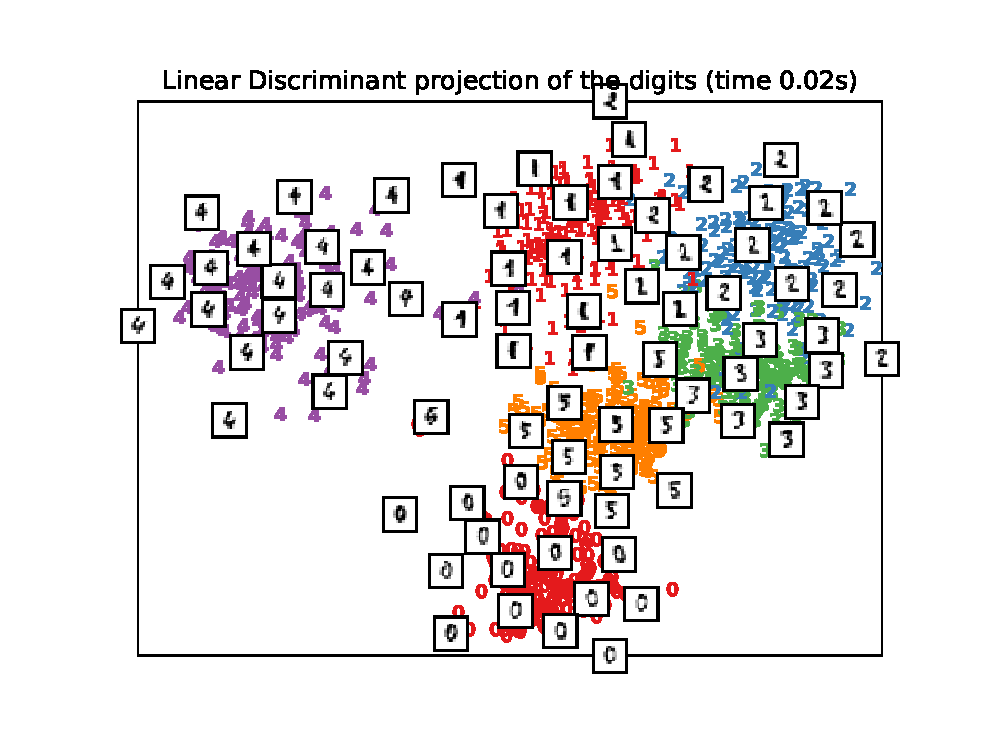
\includegraphics[scale=0.65]{./image/experiment/lda.eps}
\end{figure}
\end{frame}


\begin{frame}{Hardwriting digit visualization}
\begin{figure}
\centering
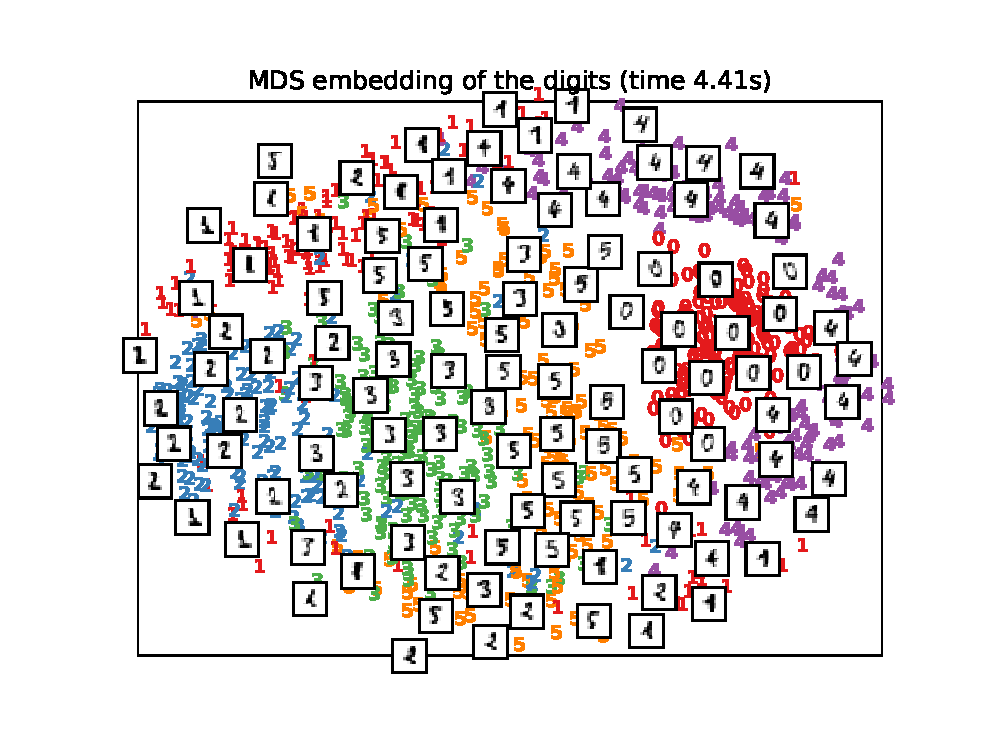
\includegraphics[scale=0.65]{./image/experiment/mds.eps}
\end{figure}
\end{frame}


\begin{frame}{Hardwriting digit visualization}
\begin{figure}
\centering
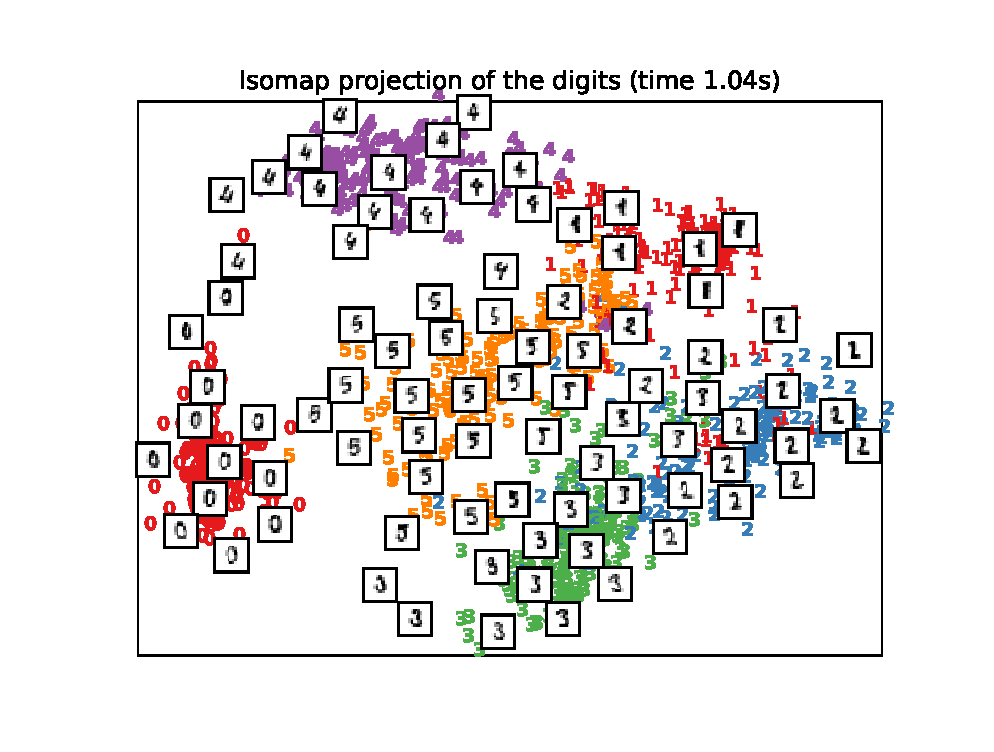
\includegraphics[scale=0.65]{./image/experiment/isomap.eps}
\end{figure}
\end{frame}

\begin{frame}{Hardwriting digit visualization}
\begin{figure}
\centering
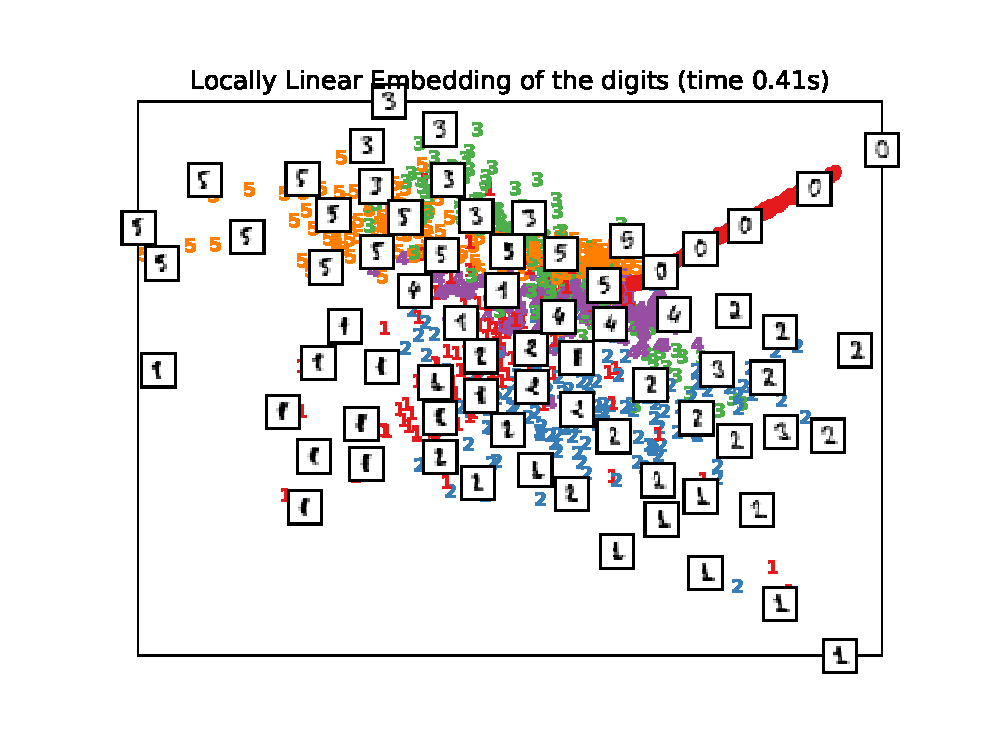
\includegraphics[scale=0.65]{./image/experiment/lle.eps}
\end{figure}
\end{frame}

\begin{frame}{Hardwriting digit visualization}
\begin{figure}
\centering
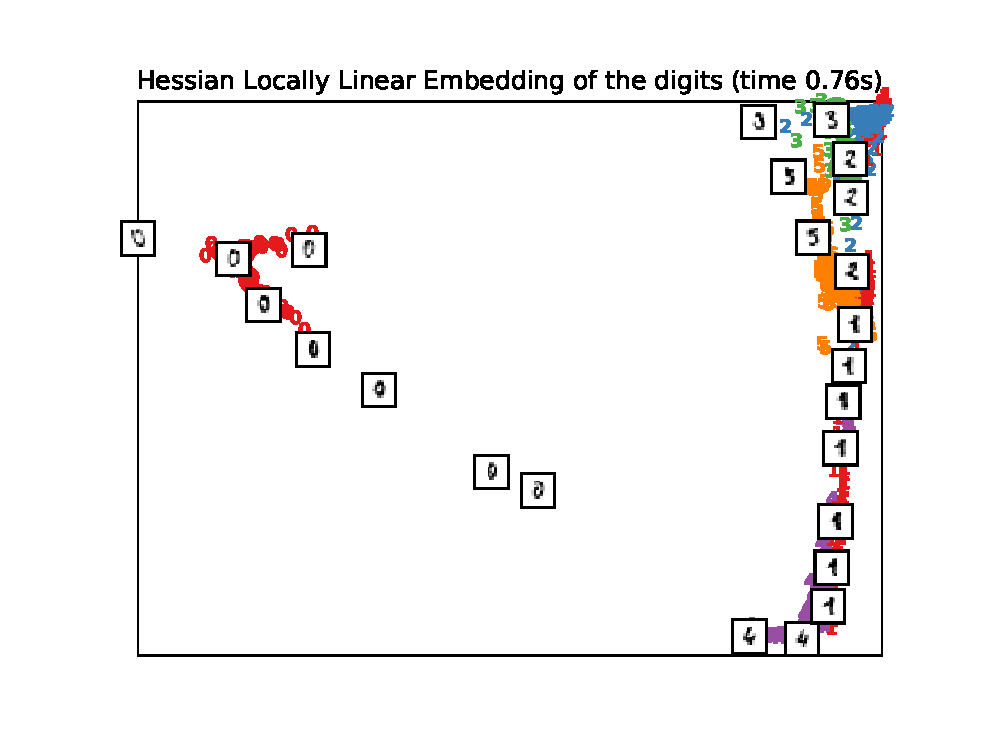
\includegraphics[scale=0.65]{./image/experiment/hlle.eps}
\end{figure}
\end{frame}

\begin{frame}{Hardwriting digit visualization}
\begin{figure}
\centering
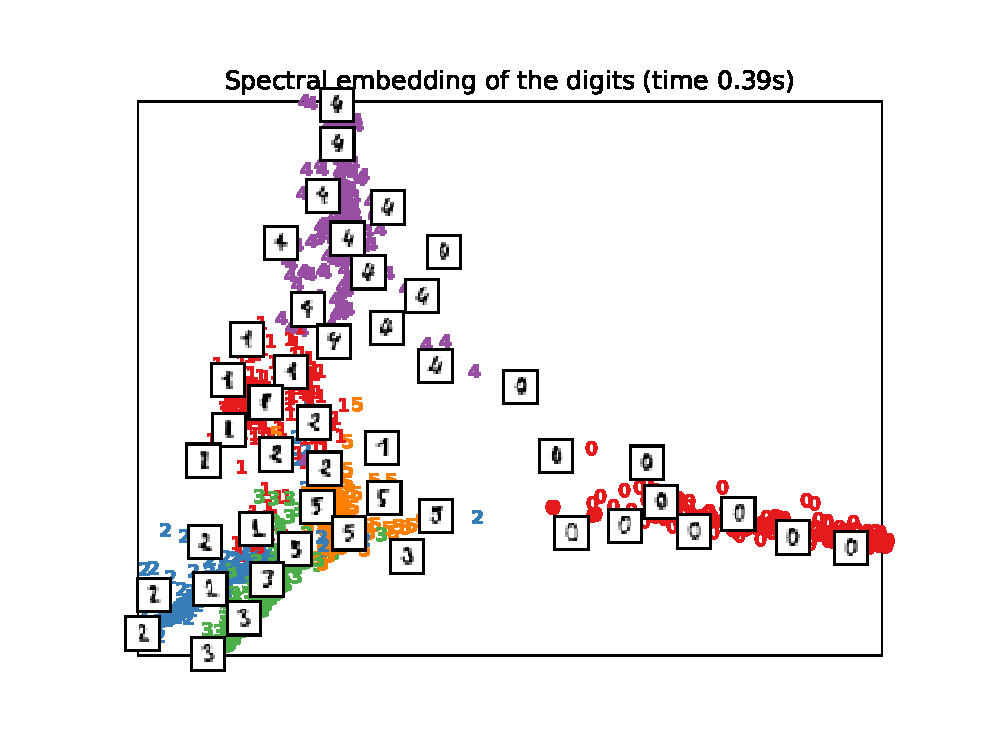
\includegraphics[scale=0.65]{./image/experiment/le.eps}
\end{figure}
\end{frame}

\begin{frame}{Hardwriting digit visualization}
\begin{figure}
\centering
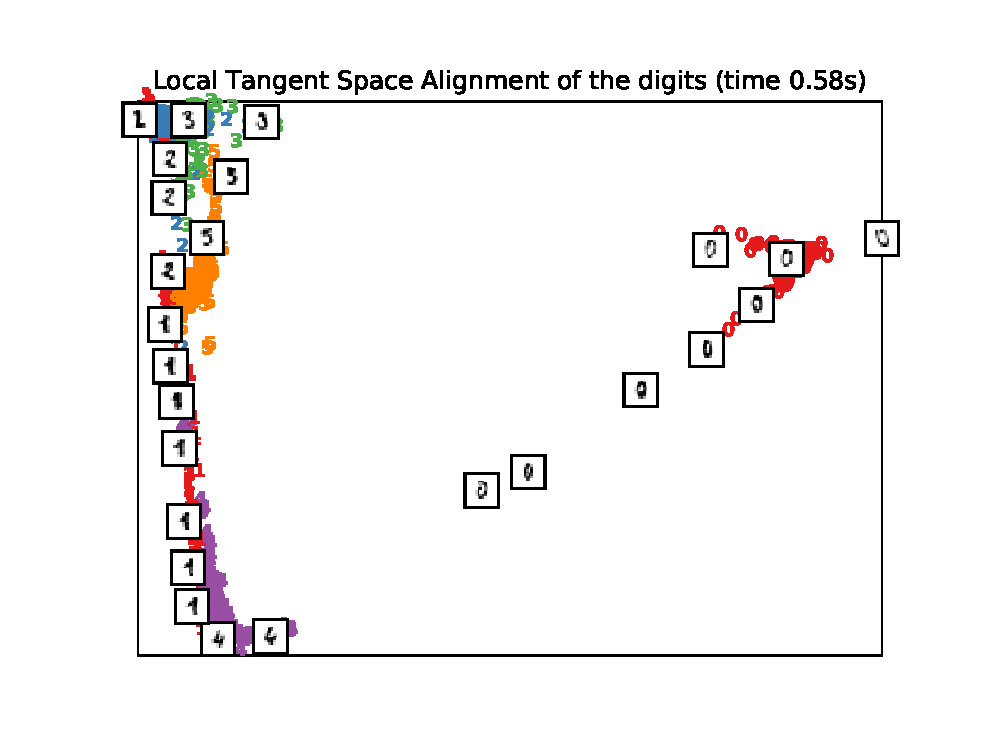
\includegraphics[scale=0.65]{./image/experiment/ltsa.eps}
\end{figure}
\end{frame}

\begin{frame}{Hardwriting digit visualization}
\begin{figure}
\centering
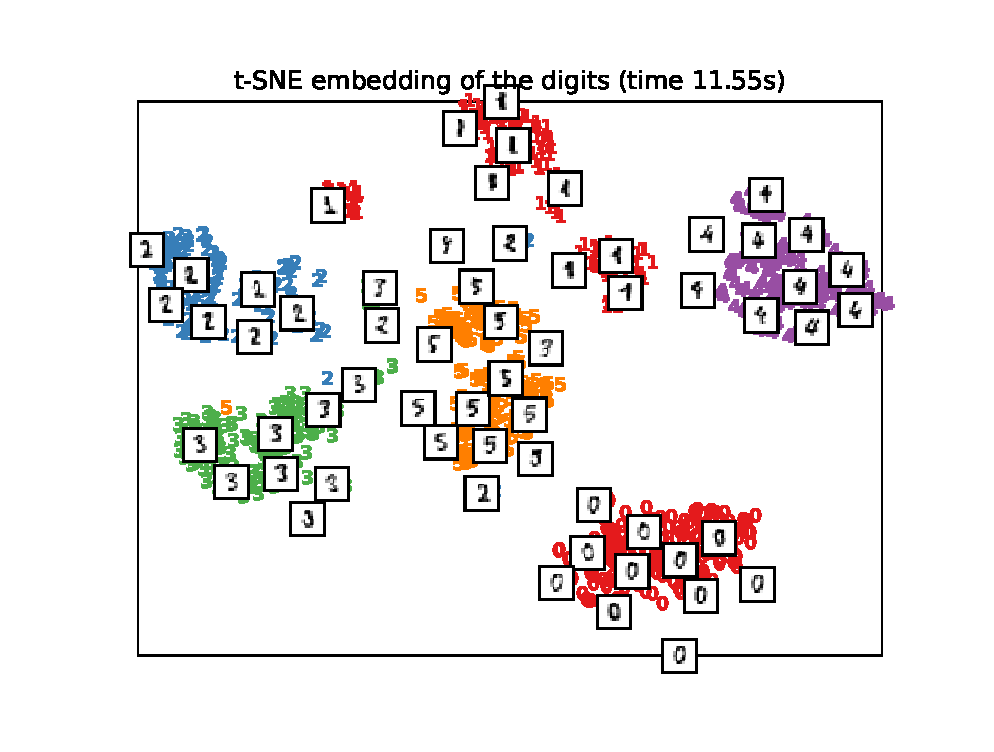
\includegraphics[scale=0.65]{./image/experiment/tsne.eps}
\end{figure}
\end{frame}


\section{Demo}
\begin{frame}{Demo}
Hero images visualization: \url{https://onefoldmedia.com/sites/default/super_t-sne}
\end{frame}

\section{Resource}
\begin{frame}{Resource}
\begin{itemize}
	\item \href{http://www.cs.toronto.edu/~hinton/absps/sne.pdf}{Stochastic Neighbor Embedding}
	\item \href{http://www.cs.toronto.edu/~hinton/absps/tsnefinal.pdf}{isualizing Data using t-SNE}
	\item \href{http://www.cs.toronto.edu/~hinton/csc2535/readings/lle.pdf}{Local Linear Embedding}
	\item \href{http://scikit-learn.org/stable/index.html}{scikit-learn}
\end{itemize}
\end{frame}

\begin{frame}{Thanks!}
\begin{center}
	\LARGE Thank you !
\end{center}
\end{frame}
\end{document}
